% Name: Tangents from an external point
% Description: The two tangents from P touch the circle at A and B, each at a right angle to the radius there, and PA = PB.
% Tags: circle theorem, tangent, radius, right angle

\usetikzlibrary{angles, calc}

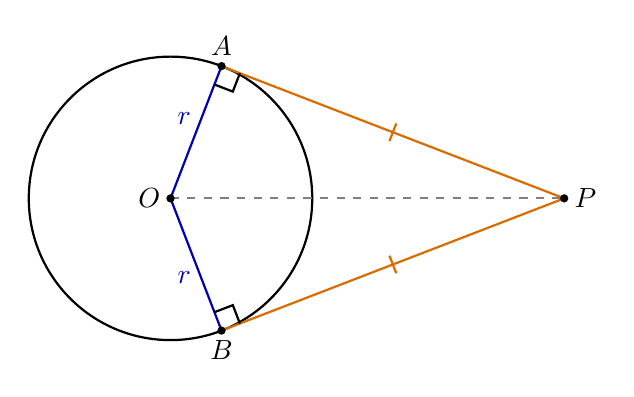
\begin{tikzpicture}[thick]
  % Tangent points: cos(angle AOP) = radius / OP = 1.8 / 5
  \pgfmathsetmacro{\t}{acos(1.8/5)}
  \coordinate[label=left:$O$] (O) at (0,0);
  \coordinate[label=right:$P$] (P) at (5,0);
  \coordinate[label=above:$A$] (A) at (\t:1.8);
  \coordinate[label=below:$B$] (B) at (-\t:1.8);
  \draw (O) circle (1.8);
  \draw[blue!70!black] (O) -- node[left, pos=0.6] {$r$} (A) (O) -- node[left, pos=0.6] {$r$} (B);
  \draw[gray, dashed] (O) -- (P);
  \draw[orange!85!black] (A) -- (P) -- (B);
  \pic[draw, angle radius=2.5mm] {right angle=O--A--P};
  \pic[draw, angle radius=2.5mm] {right angle=P--B--O};
  % Equal tick marks across the middle of each tangent
  \draw[orange!85!black] ($(A)!0.5!(P)!1.2mm!90:(P)$) -- ($(A)!0.5!(P)!1.2mm!-90:(P)$) ($(B)!0.5!(P)!1.2mm!90:(P)$) -- ($(B)!0.5!(P)!1.2mm!-90:(P)$);
  \foreach \p in {O, A, B, P} \fill (\p) circle (1.5pt);
\end{tikzpicture}
